%%%%%%%%%%%%%%%%%%%%%%%%%%%%%%%%%%%%%%%%%%%%%%%%%%%%%%%%%%%%%%%%%%%%%%%%%%%%%%%%%%
%%% Introduction
%%%%%%%%%%%%%%%%%%%%%%%%%%%%%%%%%%%%%%%%%%%%%%%%%%%%%%%%%%%%%%%%%%%%%%%%%%%%%%%%%%
\chapter{Introduction}
	\label{ch::introduction}
	
	\begin{figure}[h!]
		\centering
		\fbox{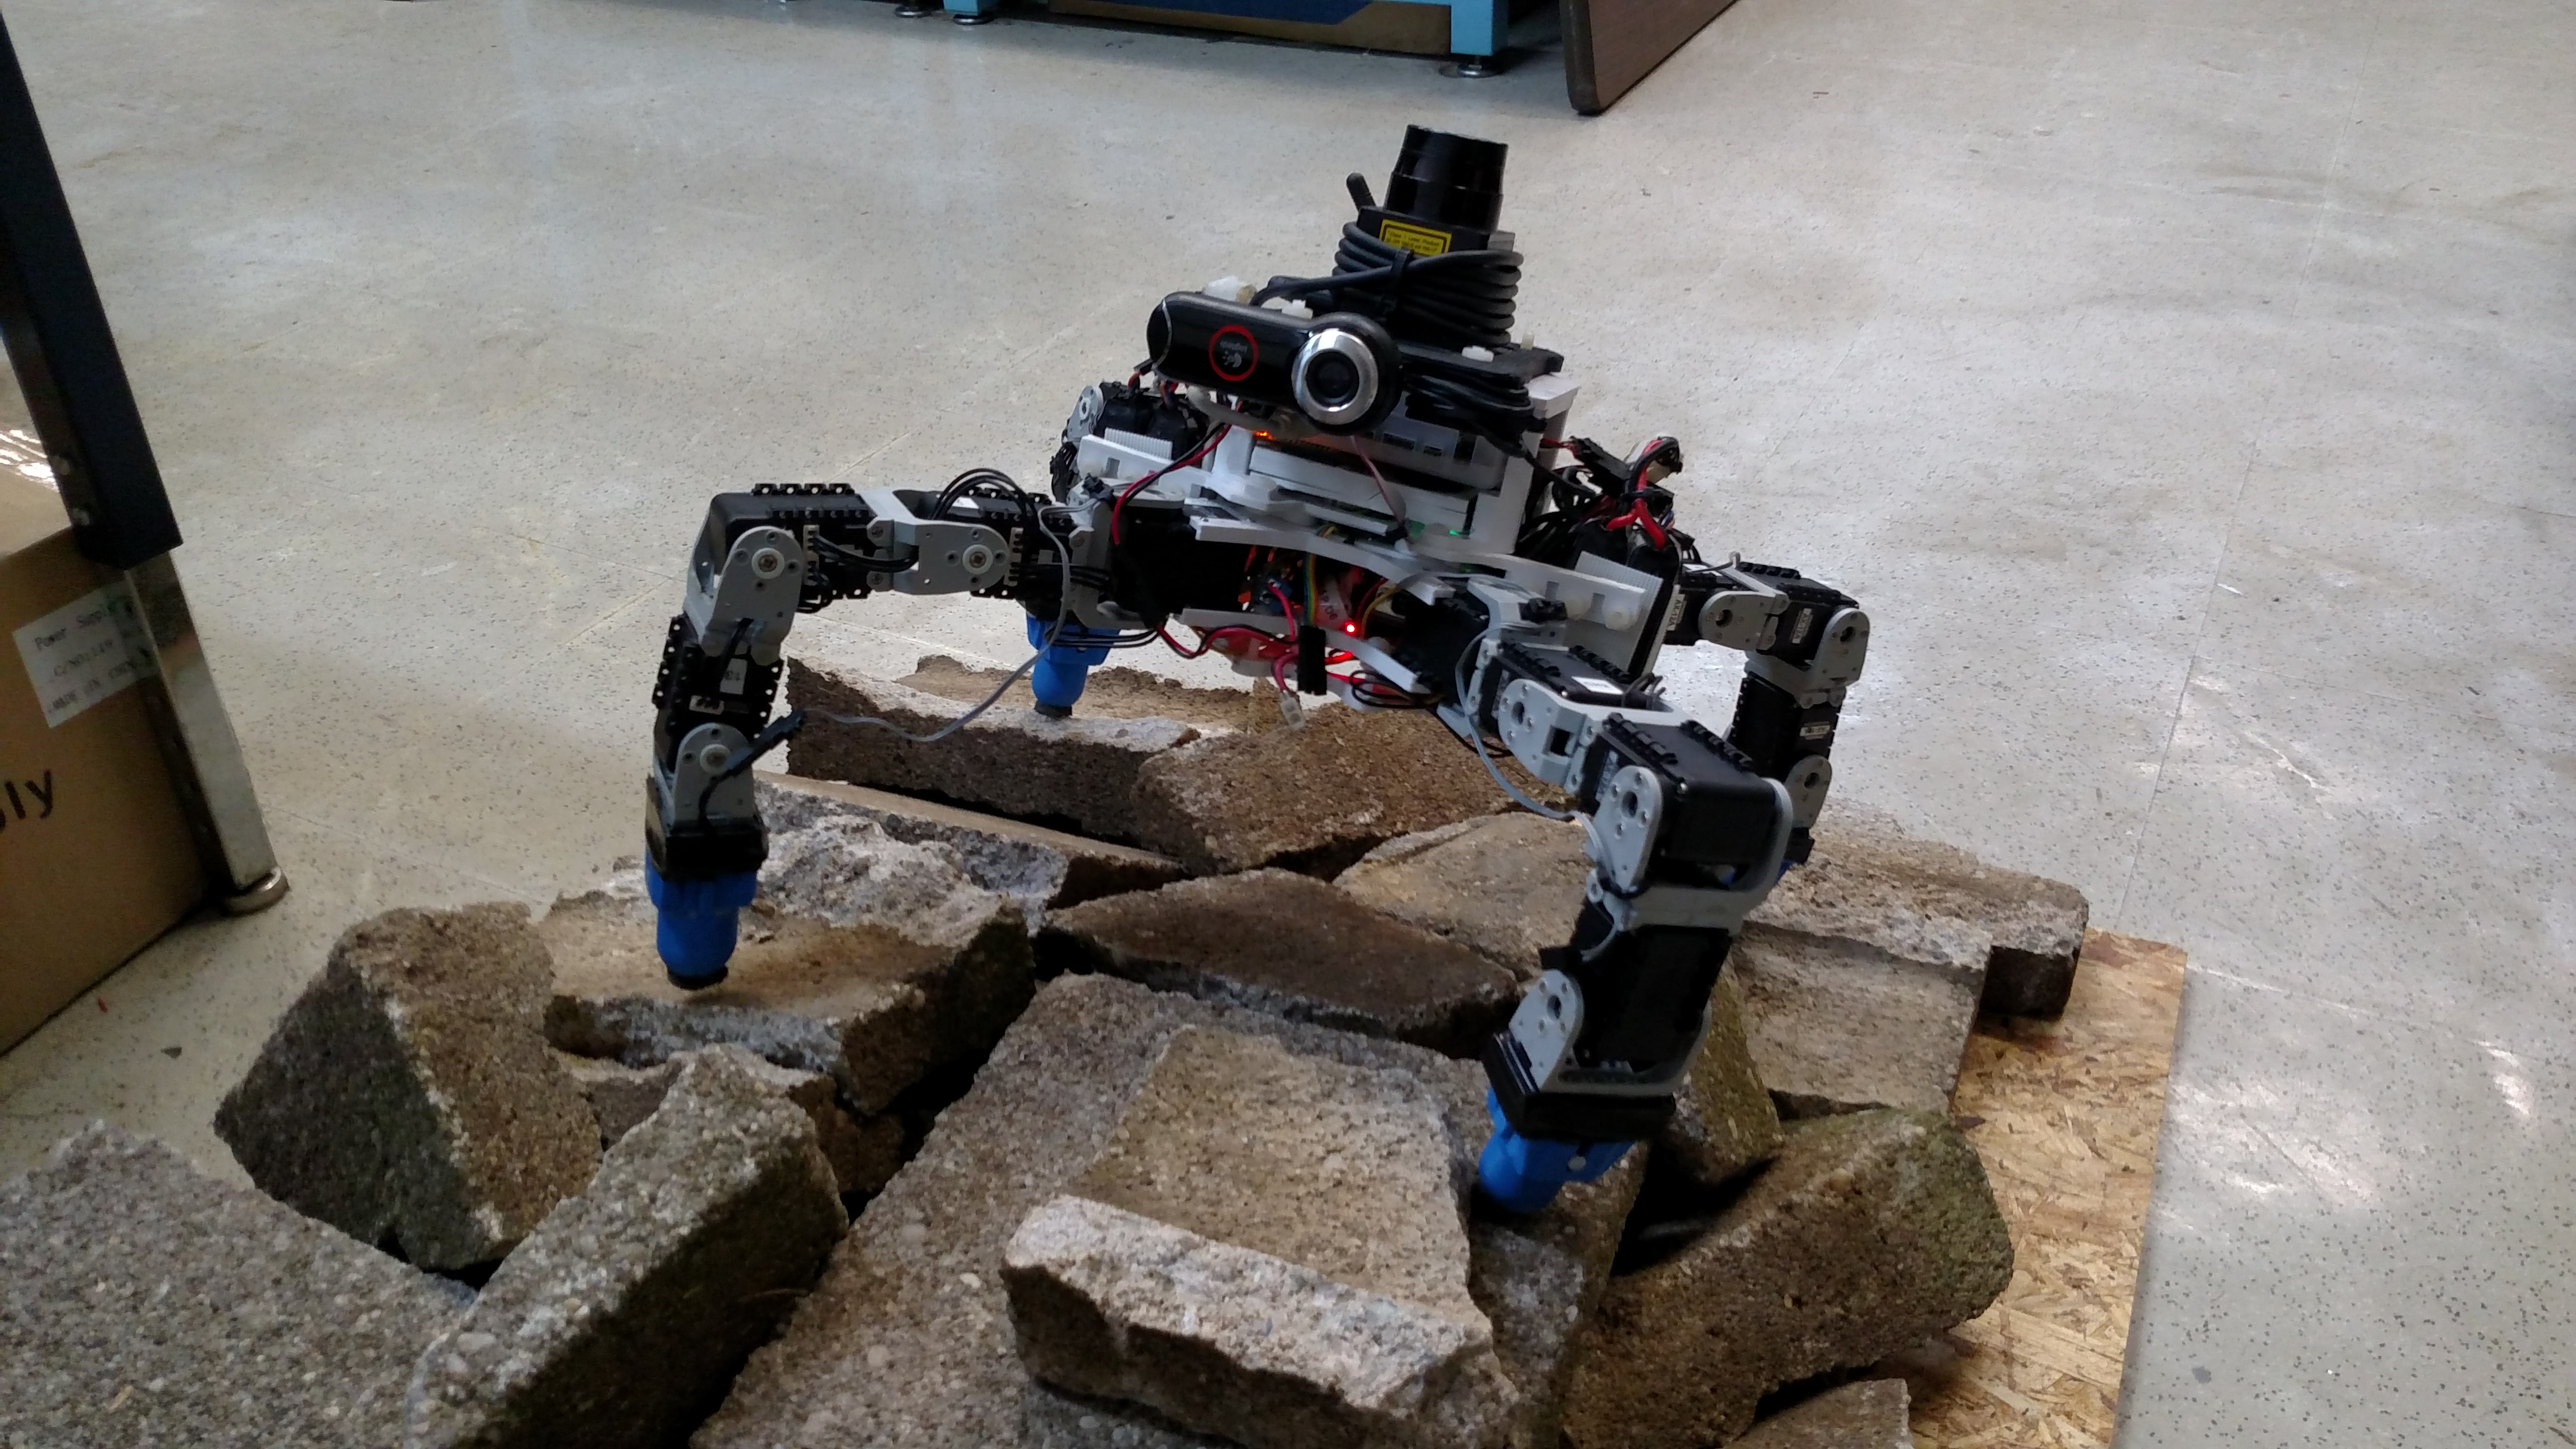
\includegraphics[width=\textwidth]{on_the_rocks2.jpg}}
		\caption{The BlueFoot Quadruped Robot}
		\label{fig::bluefoot_glamour}
	\end{figure}
		The design of legged robots and associated methods of locomotion control has been an area of interest spanning the past several decades, as shown by \cite{McGhee1965,Hodgins1991,Altendorfer2001,Kolter2008,Wieber2015}. Quadruped robotic systems have gained popularity in studies pertaining to variable terrain navigation and full-body stability adaptation. Well known examples of this from the past decade are the Tekken \cite{Fukuoka2003}, Kolt \cite{Estremera2006}, BigDog \cite{BigDog2008}, and HyQ \cite{Semini2010_PHD} quadrupeds. Many of these systems have been implemented on a larger scale so that they can carry substantial payloads while maintaining adequate system bandwidth for fast gaits and robustness to rough terrains. Few, however, have been implemented on the scale of a hobby-robot platform while still maintaining an aptitude for rough terrain navigation and comparable sensory prowess.

		The BlueFoot quadruped is a self-contained, fully-actuated platform with the dexterity to perform stabilization and repositioning maneuvers on variable terrains along the same lines as the LittleDog platform \cite{Rebula2007}. Namely, BlueFoot has been designed with 16 actuated degrees of freedom to allow for the execution of a wide range of body and leg articulation while configured in a large range of kinematic poses. This level of dexterity allows the platform to overcome raised terrain, as well as to independently control the motion of on-board sensors attached to its main trunk. Namely, BlueFoot has the ability to pitch and yaw its on-board camera and LIDAR sensor units without gaiting, simply by reposing its body. BlueFoot also includes a sizable array of other on-board sensors for feedback and control, including joint position, velocity and loading sensors; an inertial measurement unit (IMU); and foot-contact sensors. Using the computational, sensory and motor capacities at hand, BlueFoot has the ability to utilize similar control mechanisms to those implemented on larger quadruped systems, such as those previously referred to. 

		Aside from its design, the BlueFoot platform inherently demands a variety of control routines to simultaneously achieve locomotion and system stability, making this robot an ample platform for studies related to gait design and motion planning. In particular, BlueFoot's controller incorporates a large degree of kinematic modeling and open-loop gait design and stabilization for the purpose of achieving dynamic locomotion control. In particular, BlueFoot is gaited via a central pattern generator (CPG) based gaiting algorithm augmented with a foothold controller along the same lines as \cite{Ajallooeian2013} and \cite{Rutishauser2008}. Additionally, active platform stabilization is performed via a zero-moment point (ZMP) based body-posture controller which actively stabilizes the system during arbitrary gaiting sequences. The controllers presented in this thesis make use of virtual-forces to drive system reference commands. An outer-loop controller supplies commands and corrections used in system navigation control.

		As previously mentioned, BlueFoot's core gaiting routine relies on the utilization of artificial CPG's, which are inspired from biological neuro-systems which generate rhythmic motions independently of a higher-level command unit, such as a brain \cite{Ijspeert2008}. In these systems, signals emanating from independent motor units and feedback gathered from sensory neurons are utilized to trigger or inhibit a sequence of successive motor operations, creating cyclic motion patterns. In robotics, neural units take the form of multi-state unit-oscillator systems whose dynamics are coupled with other unit-oscillators within an artificial CPG network. The dynamics of these oscillators are numerically integrated on an on-board control unit and their outputs are used to drive particular degrees of freedom within the robot, such as simple joint motions. Oscillator outputs could also be used for planning periodic motions in the robot's task space which are then translated into the robot joint-space via an inverse kinematics mapping. The motions that are generated as a result of each unit-oscillator dynamics are usually coordinated, via careful programming unit-oscillator phase offsets, to perform a larger motor tasks such as walking.

		In particular, studies dealing specifically with multi-legged gaiting motions using CPG's have been carried out by \cite{Arena2001,Klaasan2002,Arena2004,Inagaki2003,Inagaki2006,Billard2000,Brambilla2006,Buchli2006,Manoonpong2007,Tsujita2001,Tsujita2004}.  In particular, \cite{Ijspeert2008} states that the attractiveness of CPG's in the control of legged robot locomotion lies in a decoupling base-robot motor control, \IE walking, from higher-level planning. Additionally, CPG's offer an effective way for smoothly switching between gaiting patterns, \EG walking, trotting, or pacing, by simply modifying only a few control parameters. As a result, the use of CPG's greatly reduces the dimensionality of the gaiting control problem by generating coordinated motions which can be modified to yield different overall motion patterns through use of only a few core parameters.

		An important aspect of the gait-design applied to the BlueFoot platform is the incorporation of feedback mechanisms, guided by the work of \cite{Fukuoka2003,Endo2004}. Namely, BlueFoot's CPG based gait generation incorporates inertial feedback signals into its CPG mechanism by using them to modify oscillator amplitudes and modulate frequencies. Additionally, instead of using a CPG to control individual quadruped joints, so as to achieve a control gait in the robot joint space, CPG outputs are used to direct foot-step trajectories and stepping patterns. This approach allows for a combination limit-cycle control methodology of classic CPG-based gaiting with some level of foot-step planning the robot's task-space, as foot-placement is explicitly prescribed via a separate planning mechanism which decoupled from the CPG gait controller. This method offers the ability to tailor CPG-based motion generation to varying terrain situations, thus merging the benefits of explicitly planned gaiting motion with the simplicity of a core gaiting routine based on CPG's.

		Because CPG-based gaits are inherently open-loop gait routines, a combination of axillary mechanisms must be used in concert with said routine to ensure gaiting and overall system stability. The aforementioned incorporation of feedback signals to modified CPG parameters is one such way this is \emph{partially} achieved on the BlueFoot robot, specifically to achieve stable gaits. While usually sufficient for stable walking over flat to moderately-uneven terrains, this method, alone, would require careful parametric tuning to work under a larger variety of environmental conditions. Thus, other means of stabilization have been incorporated into BlueFoot's gaiting routine to aid in stability.

		In particular, BlueFoot's stabilization routines make use of a concept called \emph{artificial synergy sythesis} in which gaiting is carried out independently of a stabilization routine, which is performed primarly by restricted set of the robot's degrees of freedom \cite{Vuko1972,Yamaguchi1993}. As performed in \cite{Yamaguchi1993}, adaptions to trunk motion are utilized to stabilize the overall motion of the robot utilizing a ZMP-based approach.

		Another approach to stabilization is approach has been studied with is generally opposite to those aforementioned. This approach involves a neuro-learning mechanism which is used to counter act disturbances to the quadruped system on the level of joint control so as to level the robot's top platform.
			

		This report will detail the specific implementations of each of the aforementioned control techniques		}
